%Chapter 1
\chapter{Introduction and background}  %J.H Marais, C.J.R. Kriel
\pagenumbering{arabic}
\thispagestyle{empty}
\vspace{38em}
\hrulefill
\\
\enquote*{\textit{Quote.}} - Somebody\\
\newpage

\section{Preamble}
This chapter firstly discusses background regarding deep level mining in South Africa. Next, the need to reduce costs of operation in the mining sector is examined. From this a focus in reducing energy consumption of compressed air systems is developed. Next, background on compressed air operation and energy interventions are discussed. Simulations and their value in industry is discussed leading to a problem statement and objectives of the study. Finally, an overview for the dissertation is provided.
\section{Background on deep level mining}
	\subsection{Mining profitability}
	\footnotetext[1]{inflation.eu, "Historic inflation South Africa - cpi inflation." [Online] \url{http://www.inflation.eu/inflation-rates/south-africa/historic-inflation/cpi-inflation-south-africa.aspx}, [Accessed 25 March 2017].}
	 	Various technical, economic, social and operational challenges are posing a risk to the profitability of the South African mining sector. One of the challenges the sector faces  is a rise in the cost of operation \cite{neingo2016trends}.\par
		%\paragraph*{Falling ore grades}\leavevmode\\
		A considerable factor that is contributing to the rise of operational costs in South African gold mines has been the increase in electricity costs. As shown in figure \ref{fig: Eskom tariffs}, the general cost of electricity has increased at a rate greater than inflation since 2008 \cite{Eskom2013Tariffs}.
		\begin{figure}[h!]
			\centering
			\fbox{% GNUPLOT: LaTeX picture with Postscript
\begingroup
  \makeatletter
  \providecommand\color[2][]{%
    \GenericError{(gnuplot) \space\space\space\@spaces}{%
      Package color not loaded in conjunction with
      terminal option `colourtext'%
    }{See the gnuplot documentation for explanation.%
    }{Either use 'blacktext' in gnuplot or load the package
      color.sty in LaTeX.}%
    \renewcommand\color[2][]{}%
  }%
  \providecommand\includegraphics[2][]{%
    \GenericError{(gnuplot) \space\space\space\@spaces}{%
      Package graphicx or graphics not loaded%
    }{See the gnuplot documentation for explanation.%
    }{The gnuplot epslatex terminal needs graphicx.sty or graphics.sty.}%
    \renewcommand\includegraphics[2][]{}%
  }%
  \providecommand\rotatebox[2]{#2}%
  \@ifundefined{ifGPcolor}{%
    \newif\ifGPcolor
    \GPcolortrue
  }{}%
  \@ifundefined{ifGPblacktext}{%
    \newif\ifGPblacktext
    \GPblacktextfalse
  }{}%
  % define a \g@addto@macro without @ in the name:
  \let\gplgaddtomacro\g@addto@macro
  % define empty templates for all commands taking text:
  \gdef\gplbacktext{}%
  \gdef\gplfronttext{}%
  \makeatother
  \ifGPblacktext
    % no textcolor at all
    \def\colorrgb#1{}%
    \def\colorgray#1{}%
  \else
    % gray or color?
    \ifGPcolor
      \def\colorrgb#1{\color[rgb]{#1}}%
      \def\colorgray#1{\color[gray]{#1}}%
      \expandafter\def\csname LTw\endcsname{\color{white}}%
      \expandafter\def\csname LTb\endcsname{\color{black}}%
      \expandafter\def\csname LTa\endcsname{\color{black}}%
      \expandafter\def\csname LT0\endcsname{\color[rgb]{1,0,0}}%
      \expandafter\def\csname LT1\endcsname{\color[rgb]{0,1,0}}%
      \expandafter\def\csname LT2\endcsname{\color[rgb]{0,0,1}}%
      \expandafter\def\csname LT3\endcsname{\color[rgb]{1,0,1}}%
      \expandafter\def\csname LT4\endcsname{\color[rgb]{0,1,1}}%
      \expandafter\def\csname LT5\endcsname{\color[rgb]{1,1,0}}%
      \expandafter\def\csname LT6\endcsname{\color[rgb]{0,0,0}}%
      \expandafter\def\csname LT7\endcsname{\color[rgb]{1,0.3,0}}%
      \expandafter\def\csname LT8\endcsname{\color[rgb]{0.5,0.5,0.5}}%
    \else
      % gray
      \def\colorrgb#1{\color{black}}%
      \def\colorgray#1{\color[gray]{#1}}%
      \expandafter\def\csname LTw\endcsname{\color{white}}%
      \expandafter\def\csname LTb\endcsname{\color{black}}%
      \expandafter\def\csname LTa\endcsname{\color{black}}%
      \expandafter\def\csname LT0\endcsname{\color{black}}%
      \expandafter\def\csname LT1\endcsname{\color{black}}%
      \expandafter\def\csname LT2\endcsname{\color{black}}%
      \expandafter\def\csname LT3\endcsname{\color{black}}%
      \expandafter\def\csname LT4\endcsname{\color{black}}%
      \expandafter\def\csname LT5\endcsname{\color{black}}%
      \expandafter\def\csname LT6\endcsname{\color{black}}%
      \expandafter\def\csname LT7\endcsname{\color{black}}%
      \expandafter\def\csname LT8\endcsname{\color{black}}%
    \fi
  \fi
    \setlength{\unitlength}{0.0500bp}%
    \ifx\gptboxheight\undefined%
      \newlength{\gptboxheight}%
      \newlength{\gptboxwidth}%
      \newsavebox{\gptboxtext}%
    \fi%
    \setlength{\fboxrule}{0.5pt}%
    \setlength{\fboxsep}{1pt}%
\begin{picture}(9360.00,4032.00)%
    \gplgaddtomacro\gplbacktext{%
      \colorrgb{0.00,0.00,0.00}%
      \put(682,1144){\makebox(0,0)[r]{\strut{}$0$}}%
      \colorrgb{0.00,0.00,0.00}%
      \put(682,1422){\makebox(0,0)[r]{\strut{}$5$}}%
      \colorrgb{0.00,0.00,0.00}%
      \put(682,1701){\makebox(0,0)[r]{\strut{}$10$}}%
      \colorrgb{0.00,0.00,0.00}%
      \put(682,1979){\makebox(0,0)[r]{\strut{}$15$}}%
      \colorrgb{0.00,0.00,0.00}%
      \put(682,2258){\makebox(0,0)[r]{\strut{}$20$}}%
      \colorrgb{0.00,0.00,0.00}%
      \put(682,2536){\makebox(0,0)[r]{\strut{}$25$}}%
      \colorrgb{0.00,0.00,0.00}%
      \put(682,2814){\makebox(0,0)[r]{\strut{}$30$}}%
      \colorrgb{0.00,0.00,0.00}%
      \put(682,3093){\makebox(0,0)[r]{\strut{}$35$}}%
      \colorrgb{0.00,0.00,0.00}%
      \put(682,3371){\makebox(0,0)[r]{\strut{}$40$}}%
      \colorrgb{0.00,0.00,0.00}%
      \put(814,924){\makebox(0,0){\strut{}$2006$}}%
      \colorrgb{0.00,0.00,0.00}%
      \put(2172,924){\makebox(0,0){\strut{}$2008$}}%
      \colorrgb{0.00,0.00,0.00}%
      \put(3530,924){\makebox(0,0){\strut{}$2010$}}%
      \colorrgb{0.00,0.00,0.00}%
      \put(4888,924){\makebox(0,0){\strut{}$2012$}}%
      \colorrgb{0.00,0.00,0.00}%
      \put(6246,924){\makebox(0,0){\strut{}$2014$}}%
      \colorrgb{0.00,0.00,0.00}%
      \put(7604,924){\makebox(0,0){\strut{}$2016$}}%
      \colorrgb{0.00,0.00,0.00}%
      \put(8962,924){\makebox(0,0){\strut{}$2018$}}%
    }%
    \gplgaddtomacro\gplfronttext{%
      \csname LTb\endcsname%
      \put(176,2257){\rotatebox{-270}{\makebox(0,0){\strut{}\% increase}}}%
      \put(4888,594){\makebox(0,0){\strut{}Year}}%
      \put(4888,3701){\makebox(0,0){\strut{}Electricity price increases in South Africa}}%
      \csname LTb\endcsname%
      \put(6770,393){\makebox(0,0)[r]{\strut{}Eskom general tariff increases (\%)}}%
      \csname LTb\endcsname%
      \put(1493,1562){\makebox(0,0){\strut{}6.0}}%
      \put(2172,2759){\makebox(0,0){\strut{}27.5}}%
      \put(2851,2970){\makebox(0,0){\strut{}31.3}}%
      \put(3530,2608){\makebox(0,0){\strut{}24.8}}%
      \put(4209,2664){\makebox(0,0){\strut{}25.8}}%
      \put(4888,2118){\makebox(0,0){\strut{}16.0}}%
      \put(5567,1673){\makebox(0,0){\strut{}8.0}}%
      \put(6246,1673){\makebox(0,0){\strut{}8.0}}%
      \put(6925,1673){\makebox(0,0){\strut{}8.0}}%
      \put(7604,1673){\makebox(0,0){\strut{}8.0}}%
      \put(8283,1673){\makebox(0,0){\strut{}8.0}}%
      \csname LTb\endcsname%
      \put(6770,173){\makebox(0,0)[r]{\strut{}Inflation rate in south Africa (\%)}}%
    }%
    \gplbacktext
    \put(0,0){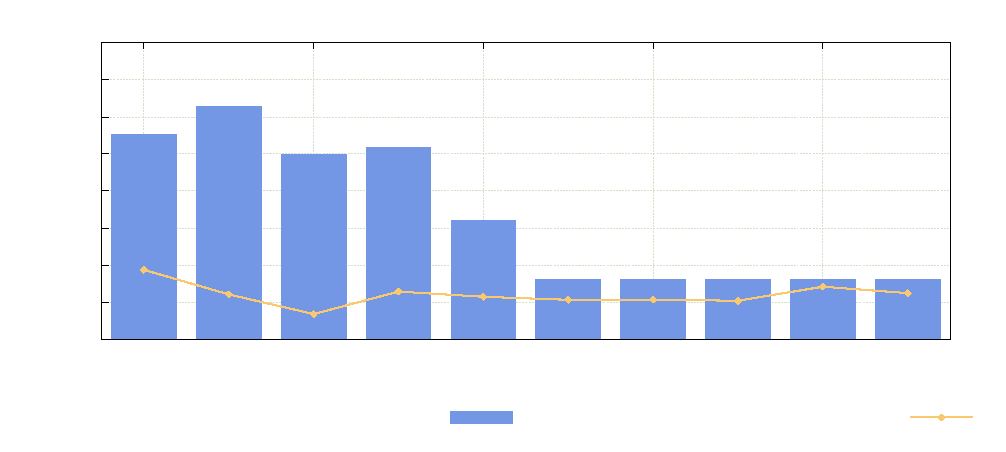
\includegraphics{Graphs/1/Eskom/Eskom}}%
    \gplfronttext
  \end{picture}%
\endgroup
}
			\caption[Electricity price increases between 2007 and 2017 compared to the inflation rate in South Africa..]{Electricity price increases between 2007 and 2017 \cite{Eskom2013Tariffs} compared to the inflation rate in South Africa.\protect\footnotemark[1] }
			\label{fig: Eskom tariffs}
		\end{figure}
		\par
		In addition to rising electricity costs, gold ore grades of South African mines have fallen substantially over the last few decades \cite{mudd2007global}. As ore grades decline, the energy utilised per unit of metal increases exponentially \cite{muller2010numerical}. Therefore mines require significantly more energy per unit of metal produced. This combination of tariff increases and increased energy usage per unit have led to significant rises in mining operation costs.
	\subsection{Process of a deep level mine}
	South Africa's mines are some of the deepest in the world Some mine shafts are reaching depths deeper then $4000m$ below the surface \cite{vosloo2012case}. The process of extracting ore at these depth is dependent on the essential services, mainly cooling and ventilation, pumping, compressed air and hoisting, as shown in figure \ref{fig: Mining Layout}.
	\par 
	 Cooling and ventilation system are required to maintain safe working temperatures underground. Pumping is critical to remove service and fissure water, preventing flooding. Compressed air is needed to safely power underground drills and machines. Finally hoisting systems are used to bring the ore to the surface and to transport mine workers in the mine. 
		\begin{figure}[h!]
			\centering
			\fbox{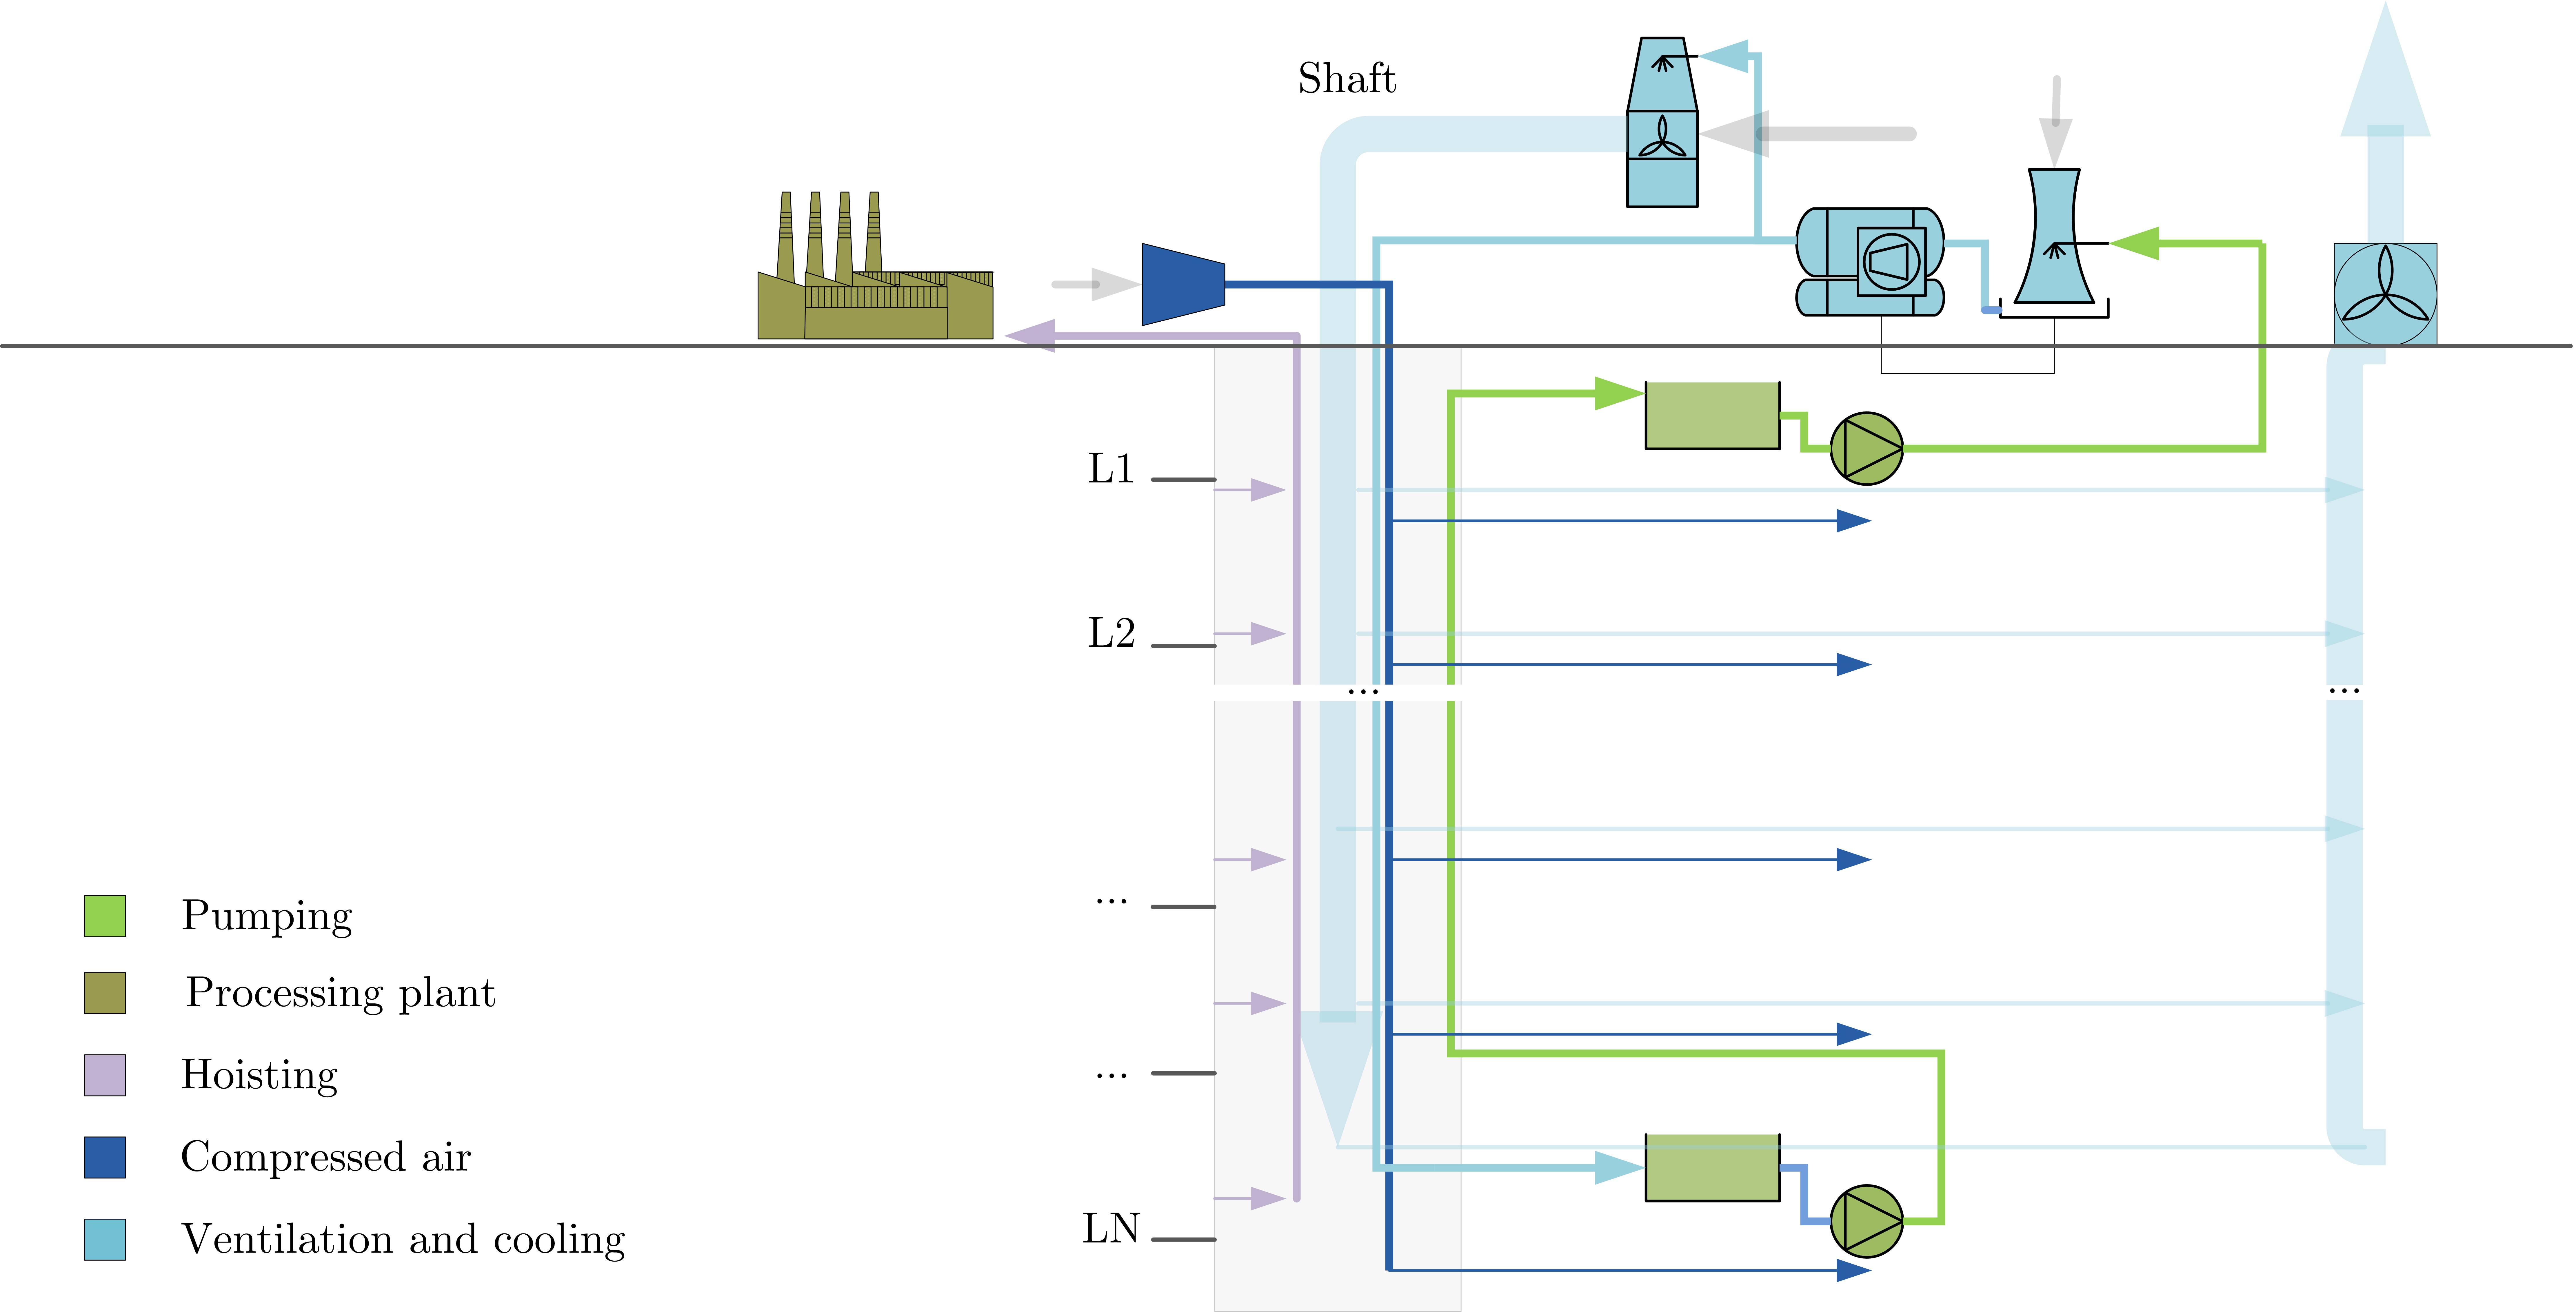
\includegraphics[width=\textwidth]{Graphs/1/Layout/Layout}}
			\caption{A layout showing the mining processes.}
			\label{fig: Mining Layout}
		\end{figure}
	\subsection{Mining Services}
		\subsubsection{Energy usage}
			The mining industry uses extensive amounts of energy. In South Africa, the industry utilizes approximately 15\% of the national electricity supplier's yearly output, of which, gold and platinum mines use 80\%.\cite{Eskom2010Energy}
			\par
			Figure \ref{fig: Energy Split} shows the division of energy within the mining industry. The chart shows that compressed air systems utilises the most energy within a mining industry. It is reasoned that energy can be most effectively reduced through the implementation of energy interventions on compressed air systems.
			\begin{figure}[h]
				\centering
				\fbox{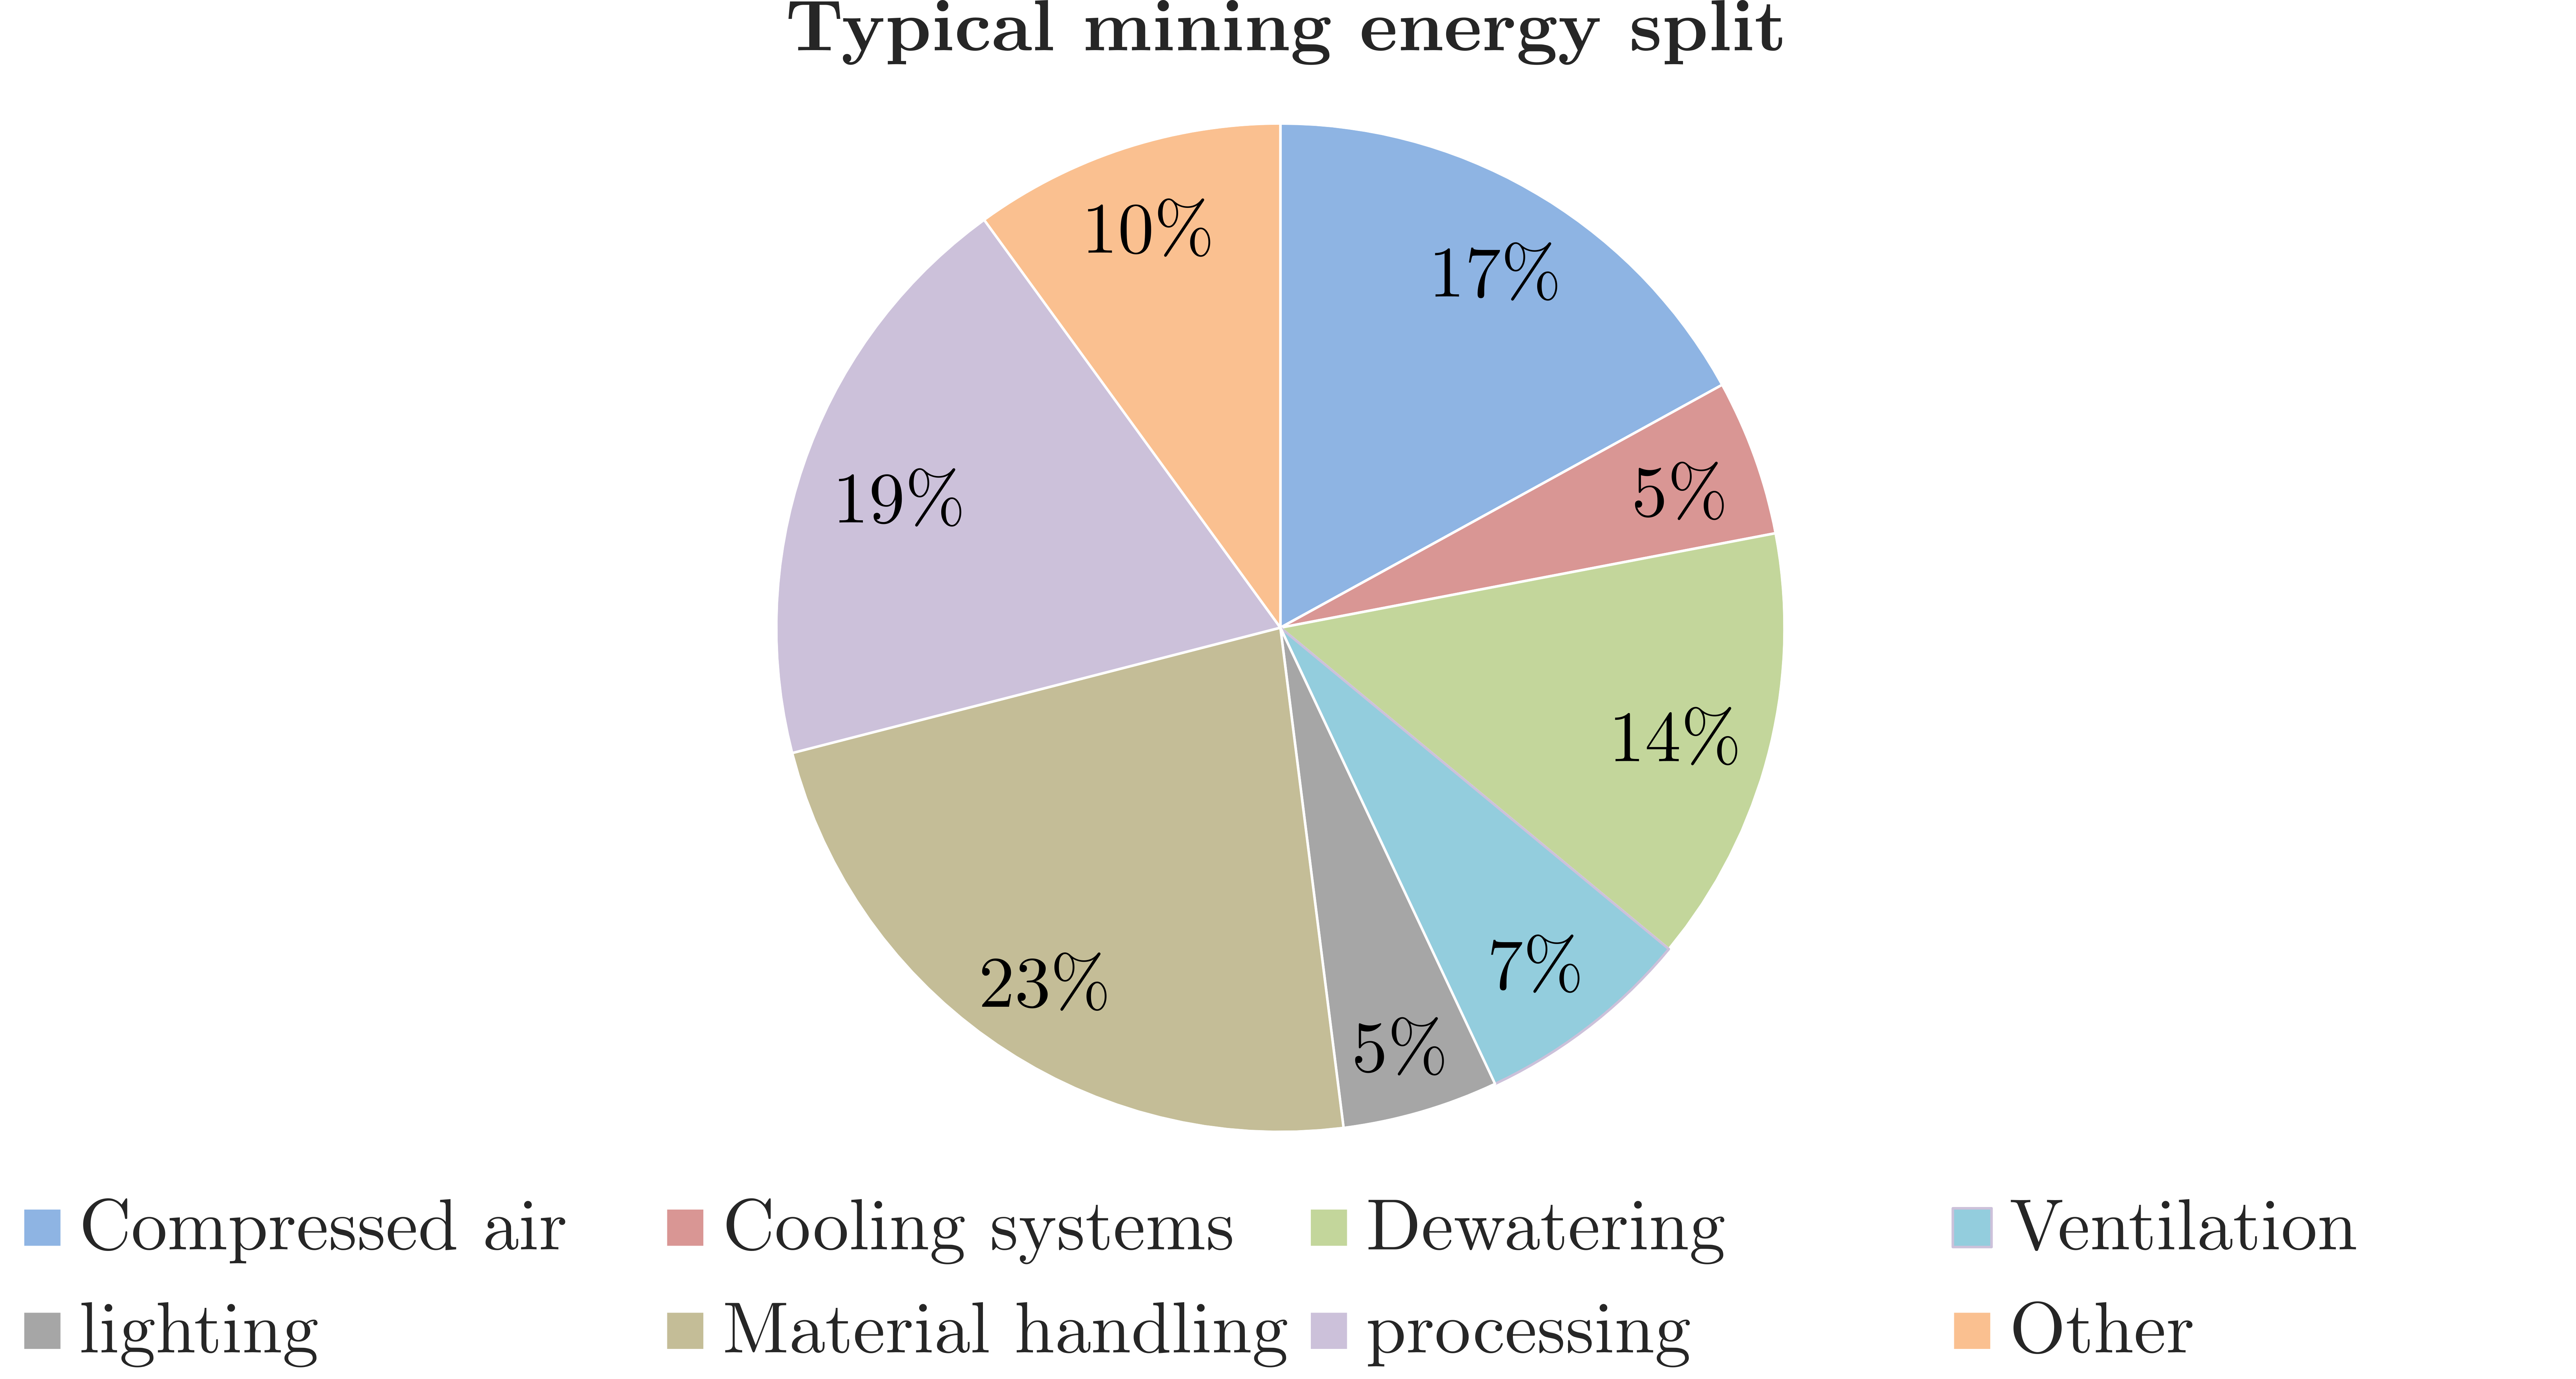
\includegraphics[ trim=-10cm -0.4cm -10cm -0.4cm,width=\textwidth]{Graphs/1/EnergySplit/EnergySplit}}
				\caption[The energy consumption for each mining system.]{The energy consumption for each mining system \cite{le2005energy}.}
				\label{fig: Energy Split}
			\end{figure}
\section{Compressed air systems in mining}
	\subsection{Compressed air in operation}\label{key}
		Largely due to their reliability, versatilely and ease of use, the South African mining industry has installed extensive compressed air networks. These systems can have compressors with capacities of up to 15 \gls{mw} \cite{Marais2012PhD}.However, the supply of compressed air is a highly energy demanding and costly process \cite{padachi2009energy}.  The energy used for compressed air production contributes to between 9\% and 20\% of the total mining energy consumption	\cite{Eskom2010Energy},\cite{du2011development}. 
		\par
		Large compressed air systems are likely inefficient. Internationally, the expected energy savings potential of a large compressed air network is 15\% \cite{neale2009compressed}. Marais \cite{marais2013simplification} showed that energy savings of up to 30\% and 40\% can be attained through various interventions. 
		\subsubsection{Pneumatic rock drills}
	 		Drilling is mainly performed in the production areas or stopes of a mine. Drill machines are used to drill holes into the rock face. Once the holes have been drilled, explosives are then installed to break up the rock \cite{van2008development}.
	 		\par
	  		Compressed air is used to power pneumatic rock drills within a mine. Pneumatic rock drills run at an efficiency of 2\%. This is low when compared to alternative rock drills such as electric, oil electro-hydraulic and hydro-powered drills that run at an efficiency of between 20-31\% \cite{fraser2008saving},\cite{vanTonder2010Masters}. 
			\subsubsection{Refuge bays}
				Refuge bays are installed in mines to provide safety to miners during emergencies. Most mines will utilise compressed air to deliver safe, cool air to the refuge bay. The provision of 1.42 $l/s$ of air per person at a pressure between 200 and 300 \gls{kpa} is required to provide oxygen and prevent any poisonousness gas entering the refuge \cite{brake1999criteria}.\par
				Airflow in the refuge bays can be controlled with a manual valve within the chamber. Any many cases, this valve is often misused by mine workers who open the valves fully in order to cool the bay through the decompression of the air. \texttt{*** need source ***}
			\subsubsection{Processing plants}
				Large processing plants are constructed near gold and mines to extract metal from the ore. These plants utilise compressed air for various systems, processes and instrumentation. Processing plants are of ten connected to the same compressed air network as the mine \cite{Marais2012PhD}. The plants use relatively low amounts of air compared to mines, however they can have pressure requirements that can complicate compressed air network optimisations .
			\subsubsection{Other compressed air usages}
			 	 Due to the availability underground, compressed air is utilised for a number of other applications. These usages include, pneumatic loaders or rock shovels, pneumatic cylinders, dam sediment agitation, cooling and ventilation and many other applications. This vast variety of of applications also leads to misuse of compressed air this leads to inefficient operation.
			\subsubsection{Operation schedule}
				On a typical mine, various operations will take place at different times of the day. Depending on the activity taking place, many mines will control the pressure to meet the requirements \cite{Kriel2014Masters},\cite{Marais2012PhD}. Figure \ref{fig: Mining schedule} shows the schedule and pressure requirement on a typical deep level mine.\par 
				As shown in the figure, the pressure requirement changes depending on the activity taking place. The drilling shift typically has the highest pressure requirement whilst blasting shift requires the lowest. Schedules and operation philosophies can differ between mines. Different operational schedules require alternative pressure requirement profiles.
				\begin{figure}[h]
					\centering
					\fbox{% GNUPLOT: LaTeX picture with Postscript
\begingroup
  \makeatletter
  \providecommand\color[2][]{%
    \GenericError{(gnuplot) \space\space\space\@spaces}{%
      Package color not loaded in conjunction with
      terminal option `colourtext'%
    }{See the gnuplot documentation for explanation.%
    }{Either use 'blacktext' in gnuplot or load the package
      color.sty in LaTeX.}%
    \renewcommand\color[2][]{}%
  }%
  \providecommand\includegraphics[2][]{%
    \GenericError{(gnuplot) \space\space\space\@spaces}{%
      Package graphicx or graphics not loaded%
    }{See the gnuplot documentation for explanation.%
    }{The gnuplot epslatex terminal needs graphicx.sty or graphics.sty.}%
    \renewcommand\includegraphics[2][]{}%
  }%
  \providecommand\rotatebox[2]{#2}%
  \@ifundefined{ifGPcolor}{%
    \newif\ifGPcolor
    \GPcolortrue
  }{}%
  \@ifundefined{ifGPblacktext}{%
    \newif\ifGPblacktext
    \GPblacktextfalse
  }{}%
  % define a \g@addto@macro without @ in the name:
  \let\gplgaddtomacro\g@addto@macro
  % define empty templates for all commands taking text:
  \gdef\gplbacktext{}%
  \gdef\gplfronttext{}%
  \makeatother
  \ifGPblacktext
    % no textcolor at all
    \def\colorrgb#1{}%
    \def\colorgray#1{}%
  \else
    % gray or color?
    \ifGPcolor
      \def\colorrgb#1{\color[rgb]{#1}}%
      \def\colorgray#1{\color[gray]{#1}}%
      \expandafter\def\csname LTw\endcsname{\color{white}}%
      \expandafter\def\csname LTb\endcsname{\color{black}}%
      \expandafter\def\csname LTa\endcsname{\color{black}}%
      \expandafter\def\csname LT0\endcsname{\color[rgb]{1,0,0}}%
      \expandafter\def\csname LT1\endcsname{\color[rgb]{0,1,0}}%
      \expandafter\def\csname LT2\endcsname{\color[rgb]{0,0,1}}%
      \expandafter\def\csname LT3\endcsname{\color[rgb]{1,0,1}}%
      \expandafter\def\csname LT4\endcsname{\color[rgb]{0,1,1}}%
      \expandafter\def\csname LT5\endcsname{\color[rgb]{1,1,0}}%
      \expandafter\def\csname LT6\endcsname{\color[rgb]{0,0,0}}%
      \expandafter\def\csname LT7\endcsname{\color[rgb]{1,0.3,0}}%
      \expandafter\def\csname LT8\endcsname{\color[rgb]{0.5,0.5,0.5}}%
    \else
      % gray
      \def\colorrgb#1{\color{black}}%
      \def\colorgray#1{\color[gray]{#1}}%
      \expandafter\def\csname LTw\endcsname{\color{white}}%
      \expandafter\def\csname LTb\endcsname{\color{black}}%
      \expandafter\def\csname LTa\endcsname{\color{black}}%
      \expandafter\def\csname LT0\endcsname{\color{black}}%
      \expandafter\def\csname LT1\endcsname{\color{black}}%
      \expandafter\def\csname LT2\endcsname{\color{black}}%
      \expandafter\def\csname LT3\endcsname{\color{black}}%
      \expandafter\def\csname LT4\endcsname{\color{black}}%
      \expandafter\def\csname LT5\endcsname{\color{black}}%
      \expandafter\def\csname LT6\endcsname{\color{black}}%
      \expandafter\def\csname LT7\endcsname{\color{black}}%
      \expandafter\def\csname LT8\endcsname{\color{black}}%
    \fi
  \fi
    \setlength{\unitlength}{0.0500bp}%
    \ifx\gptboxheight\undefined%
      \newlength{\gptboxheight}%
      \newlength{\gptboxwidth}%
      \newsavebox{\gptboxtext}%
    \fi%
    \setlength{\fboxrule}{0.5pt}%
    \setlength{\fboxsep}{1pt}%
\begin{picture}(9360.00,4032.00)%
    \gplgaddtomacro\gplbacktext{%
      \colorrgb{0.00,0.00,0.00}%
      \put(814,1364){\makebox(0,0)[r]{\strut{}$400$}}%
      \colorrgb{0.00,0.00,0.00}%
      \put(814,1615){\makebox(0,0)[r]{\strut{}$420$}}%
      \colorrgb{0.00,0.00,0.00}%
      \put(814,1866){\makebox(0,0)[r]{\strut{}$440$}}%
      \colorrgb{0.00,0.00,0.00}%
      \put(814,2117){\makebox(0,0)[r]{\strut{}$460$}}%
      \colorrgb{0.00,0.00,0.00}%
      \put(814,2368){\makebox(0,0)[r]{\strut{}$480$}}%
      \colorrgb{0.00,0.00,0.00}%
      \put(814,2618){\makebox(0,0)[r]{\strut{}$500$}}%
      \colorrgb{0.00,0.00,0.00}%
      \put(814,2869){\makebox(0,0)[r]{\strut{}$520$}}%
      \colorrgb{0.00,0.00,0.00}%
      \put(814,3120){\makebox(0,0)[r]{\strut{}$540$}}%
      \colorrgb{0.00,0.00,0.00}%
      \put(814,3371){\makebox(0,0)[r]{\strut{}$560$}}%
      \colorrgb{0.00,0.00,0.00}%
      \put(946,1232){\rotatebox{-270}{\makebox(0,0)[r]{\strut{}00:00}}}%
      \colorrgb{0.00,0.00,0.00}%
      \put(1295,1232){\rotatebox{-270}{\makebox(0,0)[r]{\strut{}01:00}}}%
      \colorrgb{0.00,0.00,0.00}%
      \put(1643,1232){\rotatebox{-270}{\makebox(0,0)[r]{\strut{}02:00}}}%
      \colorrgb{0.00,0.00,0.00}%
      \put(1992,1232){\rotatebox{-270}{\makebox(0,0)[r]{\strut{}03:00}}}%
      \colorrgb{0.00,0.00,0.00}%
      \put(2340,1232){\rotatebox{-270}{\makebox(0,0)[r]{\strut{}04:00}}}%
      \colorrgb{0.00,0.00,0.00}%
      \put(2689,1232){\rotatebox{-270}{\makebox(0,0)[r]{\strut{}05:00}}}%
      \colorrgb{0.00,0.00,0.00}%
      \put(3037,1232){\rotatebox{-270}{\makebox(0,0)[r]{\strut{}06:00}}}%
      \colorrgb{0.00,0.00,0.00}%
      \put(3386,1232){\rotatebox{-270}{\makebox(0,0)[r]{\strut{}07:00}}}%
      \colorrgb{0.00,0.00,0.00}%
      \put(3734,1232){\rotatebox{-270}{\makebox(0,0)[r]{\strut{}08:00}}}%
      \colorrgb{0.00,0.00,0.00}%
      \put(4083,1232){\rotatebox{-270}{\makebox(0,0)[r]{\strut{}09:00}}}%
      \colorrgb{0.00,0.00,0.00}%
      \put(4431,1232){\rotatebox{-270}{\makebox(0,0)[r]{\strut{}10:00}}}%
      \colorrgb{0.00,0.00,0.00}%
      \put(4780,1232){\rotatebox{-270}{\makebox(0,0)[r]{\strut{}11:00}}}%
      \colorrgb{0.00,0.00,0.00}%
      \put(5128,1232){\rotatebox{-270}{\makebox(0,0)[r]{\strut{}12:00}}}%
      \colorrgb{0.00,0.00,0.00}%
      \put(5477,1232){\rotatebox{-270}{\makebox(0,0)[r]{\strut{}13:00}}}%
      \colorrgb{0.00,0.00,0.00}%
      \put(5825,1232){\rotatebox{-270}{\makebox(0,0)[r]{\strut{}14:00}}}%
      \colorrgb{0.00,0.00,0.00}%
      \put(6174,1232){\rotatebox{-270}{\makebox(0,0)[r]{\strut{}15:00}}}%
      \colorrgb{0.00,0.00,0.00}%
      \put(6522,1232){\rotatebox{-270}{\makebox(0,0)[r]{\strut{}16:00}}}%
      \colorrgb{0.00,0.00,0.00}%
      \put(6871,1232){\rotatebox{-270}{\makebox(0,0)[r]{\strut{}17:00}}}%
      \colorrgb{0.00,0.00,0.00}%
      \put(7219,1232){\rotatebox{-270}{\makebox(0,0)[r]{\strut{}18:00}}}%
      \colorrgb{0.00,0.00,0.00}%
      \put(7568,1232){\rotatebox{-270}{\makebox(0,0)[r]{\strut{}19:00}}}%
      \colorrgb{0.00,0.00,0.00}%
      \put(7916,1232){\rotatebox{-270}{\makebox(0,0)[r]{\strut{}20:00}}}%
      \colorrgb{0.00,0.00,0.00}%
      \put(8265,1232){\rotatebox{-270}{\makebox(0,0)[r]{\strut{}21:00}}}%
      \colorrgb{0.00,0.00,0.00}%
      \put(8613,1232){\rotatebox{-270}{\makebox(0,0)[r]{\strut{}22:00}}}%
      \colorrgb{0.00,0.00,0.00}%
      \put(8962,1232){\rotatebox{-270}{\makebox(0,0)[r]{\strut{}23:00}}}%
    }%
    \gplgaddtomacro\gplfronttext{%
      \csname LTb\endcsname%
      \put(176,2367){\rotatebox{-270}{\makebox(0,0){\strut{}kPa}}}%
      \put(4954,374){\makebox(0,0){\strut{}Time of day}}%
      \put(4954,3701){\makebox(0,0){\strut{}Typical mining schedule and pressure requirement}}%
      \csname LTb\endcsname%
      \put(6242,173){\makebox(0,0)[r]{\strut{}Pressure requirement (kPa)}}%
      \csname LTb\endcsname%
      \put(1817,2368){\rotatebox{-270}{\makebox(0,0){\strut{}\shortstack{Sweeping and \\ cleaning}}}}%
      \put(3037,2368){\rotatebox{-270}{\makebox(0,0){\strut{}\shortstack{Workers travel to \\ working areas}}}}%
      \put(4605,2368){\makebox(0,0){\strut{}\shortstack{Drilling}}}%
      \put(6174,2368){\rotatebox{-270}{\makebox(0,0){\strut{}\shortstack{Explosive charge \\ up}}}}%
      \put(7394,2368){\makebox(0,0){\strut{}\shortstack{Blasting}}}%
      \put(8613,2368){\rotatebox{-270}{\makebox(0,0){\strut{}\shortstack{Sweeping and \\ cleaning}}}}%
    }%
    \gplbacktext
    \put(0,0){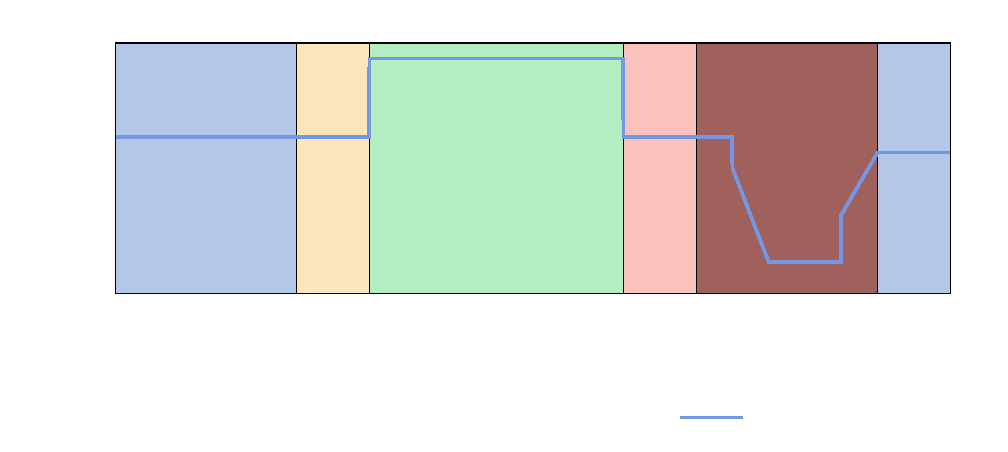
\includegraphics{Graphs/1/MiningSchedule/MiningSchedule}}%
    \gplfronttext
  \end{picture}%
\endgroup
}
					\caption[A typical operation schedule of a deep level mine.]{The typical operation schedule of a deep level mine \cite{Kriel2014Masters}.}
					\label{fig: Mining schedule}
				\end{figure}
	\subsection{Characteristic inefficiencies of compressed air systems}
		Compressed air distribution networks in the mining industry consist of multiple compressors and working areas up to eight kilometres away from the source \cite{Marais2012PhD}. Due to their size and complexity, these systems are prone to large energy losses.
		\par 
		Compressed air leakage accounts for as much as 35\% of the energy losses of a compressed air network \cite{Lawrence2004Improving}. Other systemic losses include, faulty valves, pipe diameter fluctuations, obstructed air compressor intake filters and inefficient compressors. 	
		\subsection{Instrumentation and measurements}
		For large industrial systems, thorough instrumentation is necessary in order to monitor performance and equipment condition throughout the system. In a mining compressed air network, instrumentation is installed to monitor flows, pressures, temperatures ,etc.. Electrical instrumentation is also installed for sensing currents, power factors, voltages and power. On control valves, input/output pressures, flows and valve position are usually measured with instrumentation.	
		\par
		 A \gls{scada} system is used to monitor and control processes throughout the mine from a control room. The \gls{scada} centralises instrumentation data from \glspl{plc} throughout the mine. The \gls{scada} can also be used to control machines and instrumentation by sending control signals to the relevant \gls{plc}.  Communication to the underground \glspl{plc} is achieved using a substantial fibre optic network.\cite{schroeder2009energy}

	\subsection{Inefficiency identification methods}
		Leakage and inefficiency detection strategies is not often pursued in the South African mining industry \cite{vanTonder2010Masters}. Many mines do however perform leak inspections either internally or by a outside company. In these inspections, an ultrasonic detector is used to locate the leak. Alternatively, some mines employ the \enquote{walk and listen} method to identify leaks from the audible sound that it produces \cite{vanTonder2010Masters}. Once the inspection is completed, the findings, including the locations and estimated costs of all identified leaks, are reported.
	\subsection{Compressed air savings strategies}
		Strategies to reduce energy on compressed air systems can be summarised as follows \cite{Snyman2011Masters}:
		\begin{itemize}
			\item Reducing leaks.
			\item Reducing demand.
			\item Reducing unauthorised usage.
			\item Increasing supply efficiency.
			\item Optimising supply.
		\end{itemize}
	Often a combination of energy strategies will lead to the most savings \cite{Marais2012PhD}. Specific energy saving measures that have successfully reduced energy on mine compressed air systems will be discussed in Chapter 2.
	\section{Use of simulation in industry }
	\subsection{Background in industrial simulation}
		Continuous improvements in computing hardware has led to major advancement in software technology. Consequently the use of computational simulation has become an increasingly valuable tool for many industries.\cite{kocsis2003integration} \par 
		In \textit{ Handbook of simulation: principles, methodology, advances, applications, and practice}, the advantages of the use of simulation in industry are discussed as follows \cite{banks1998handbook}: 
		\begin{itemize}
			\item The ability to test new policies, operating procedures and methods without causing a disruption to the actual system.
			\item The means to identify problems in complex systems by gathering insight in the interactions within the system.
			\item The facility to compress or expand time to investigate phenomena thoroughly.
			\item The capability to determine the limits and constraints within a system.
			\item The potential to build consensus with regard to proposed designs or modifications.
		\end{itemize}

	\subsection{Simulation usage in mining}
		Simulation has been used to test and identify energy and operational improvements in mining systems. However,  existing tools required to much data to model the systems accurately, [CITATION NEEDED] Resulting in simplified simulation models.  New tools such the \gls{stb} software, have made it possible to develop highly accurate, detailed simulations for mining systems. This will alolow more complex intervention to be tested with more accuracy.
		
	\section{Problem statement and objectives}
	\subsection{Problem statement}
 		Rising costs and falling ore grades are driving in the mining industry to reduce operational inefficiencies. Large energy savings can be made in Compressed air systems in the mining industry. However manual testing of interventions can be cumbersome.
 		\par
 		Computer modeling and simulation of compressed air systems can be used to quantify and priorities operational interventions that improve efficiency. These interventions can be evaluated with minimal risk. However simulations have not been utilized to their full potential in the mining industry. With new tools that allow for more detailed simulation models of mining systems could allow for of identification of more effective energy savings measures for mines.
	\subsection{Research objectives}
		The main objective of this dissertation is achieve energy savings and identify operational improvements in mining compressed air systems. A simulation process to will be developed to achieve this goal.
\section{Dissertation overview}
	\texttt{Describe (in approximately one sentence each) the contents of \\each of the dissertation chapters. No results here.}